% Mid-semester research project milestone: one-page A4 summary.
%
% Uses Trebuchet MS, so it must be compiled with a Unicode engine:
%   tools\tectonic.exe milestone\midsemester_summary.tex    (or run build.bat)
%   xelatex / lualatex also work; pdflatex does not.
% The four Trebuchet MS font files are read from the fonts/ folder beside this file
% (copied from C:/Windows/Fonts/).

\documentclass[10pt,a4paper]{article}

\usepackage{fontspec}
\setmainfont{trebuc.ttf}[
  Path           = fonts/,
  BoldFont       = trebucbd.ttf,
  ItalicFont     = trebucit.ttf,
  BoldItalicFont = trebucbi.ttf,
  Ligatures      = TeX]
\usepackage[a4paper,left=1.3cm,right=1.3cm,top=1.0cm,bottom=0.9cm]{geometry}
\usepackage{xcolor}
\usepackage{enumitem}
\usepackage{tikz}
\usetikzlibrary{positioning,calc}

\pagestyle{empty}
\setlength{\parindent}{0pt}
\setlength{\parskip}{2pt}
\linespread{0.98}
\setlist[itemize]{leftmargin=1.05em, itemsep=0.8pt, topsep=1pt, parsep=0pt, partopsep=0pt, label=\textbullet}

\definecolor{accent}{HTML}{2E6DA4}
\definecolor{boxfill}{HTML}{EEF3F8}
\definecolor{boxline}{HTML}{5B7FA6}
\definecolor{newfill}{HTML}{FFF1D6}
\definecolor{newline}{HTML}{C77700}

\newcommand{\head}[1]{\par\vspace{4pt}{\bfseries\color{accent}\fontsize{10.4}{12}\selectfont #1}\par\vspace{0.5pt}}
\newcommand{\lead}[1]{\textbf{#1}}
\newcommand{\new}{\textcolor{newline}{\bfseries NEW}}

\begin{document}

{\bfseries\fontsize{13}{15}\selectfont MID-SEMESTER RESEARCH PROJECT MILESTONE: ONE-PAGE SUMMARY}\par
\vspace{3pt}{\color{accent}\hrule height 1pt}\vspace{4pt}

\lead{Student:} Opol Charis \;|\; \lead{Registration No.:} S24B23/003 \;|\; \lead{Access No.:} B29654 \;|\; \lead{Programme:} BSc Computer Science

\vspace{1pt}
{\bfseries\fontsize{11}{13}\selectfont Title: Rule-Constrained Reinforcement Learning for Ambiguity-Aware IT Incident Triage}

\head{Problem and research objective}
\lead{Problem.} When an IT incident is reported, support staff must act before they know the cause, and the first evidence is often incomplete or contradictory. They can check further, try a likely fix, or pass the incident to another technician. Current AI tools give one answer per ticket. They cannot ask for more evidence or signal that they are unsure~[1].

\lead{Objective.} To build and test an AI agent that learns when to check further, when to recommend a fix that the rules allow, and when to hand the incident to a human technician.

\head{What exists, the gap and my contribution}
\lead{What exists.}
\begin{itemize}
  \item AI tools sort tickets using the report alone, but symptoms often do not reveal the cause, so tickets are passed between teams several times~[1].
  \item ``Shielding'' stops a learning agent from breaking set rules, but it has been tested mainly on robots and games~[2].
  \item ``Learning to defer'' passes hard cases to a person, but gives no option to gather more evidence first~[3].
\end{itemize}
\lead{Gap.} In the 46 sources I reviewed, these ideas appear only two at a time. No study puts all three choices in one agent for IT incidents, checks it against rules, and tests it as the evidence gets worse.

\lead{Contribution.} (1)~A simulator of IT incidents in which the quality of the evidence can be turned up or down. (2)~An agent with the three choices and a separate rule checker. (3)~A fair comparison with six simpler strategies on four measures, not accuracy alone.

\head{Full research pipeline}
\vspace{1pt}
\begin{center}
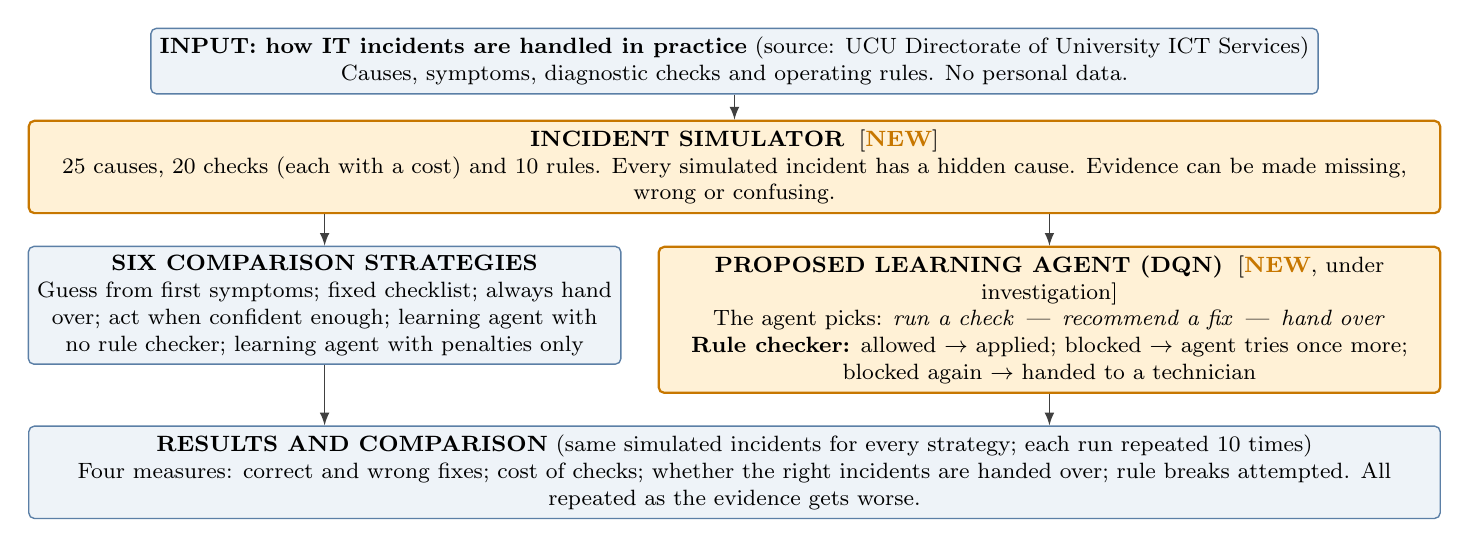
\begin{tikzpicture}[
  font=\fontsize{8}{9.7}\selectfont,
  box/.style={draw=boxline, fill=boxfill, rounded corners=2pt, line width=0.5pt, align=flush center, inner sep=3.2pt},
  newbox/.style={box, draw=newline, fill=newfill, line width=0.8pt},
  arr/.style={-latex, line width=0.6pt, draw=black!75}]
  \node[box, text width=14.6cm] (input) {\textbf{INPUT: how IT incidents are handled in practice} (source: UCU Directorate of University ICT Services)\\
    Causes, symptoms, diagnostic checks and operating rules. No personal data.};
  \node[newbox, text width=17.7cm, below=3.2mm of input] (env) {\textbf{INCIDENT SIMULATOR} \;[\new]\\
    25 causes, 20 checks (each with a cost) and 10 rules. Every simulated incident has a hidden cause.
    Evidence can be made missing, wrong or confusing.};
  \node[box, text width=7.3cm, anchor=north west] (base) at ($(env.south west)+(0,-4mm)$) {\textbf{SIX COMPARISON STRATEGIES}\\
    Guess from first symptoms; fixed checklist; always hand over; act when confident enough; learning agent with no rule checker; learning agent with penalties only};
  \node[newbox, text width=9.7cm, anchor=north east] (agent) at ($(env.south east)+(0,-4mm)$) {\textbf{PROPOSED LEARNING AGENT (DQN)} \;[\new, under investigation]\\
    The agent picks: \emph{run a check} \,|\, \emph{recommend a fix} \,|\, \emph{hand over}\\
    \textbf{Rule checker:} allowed $\rightarrow$ applied; blocked $\rightarrow$ agent tries once more;\\ blocked again $\rightarrow$ handed to a technician};
  \path let \p1=(base.south), \p2=(agent.south) in coordinate (lowy) at (0,{min(\y1,\y2)});
  \node[box, text width=17.7cm, anchor=north] (out) at ($(env.south |- lowy) + (0,-4mm)$) {\textbf{RESULTS AND COMPARISON} (same simulated incidents for every strategy; each run repeated 10 times)\\
    Four measures: correct and wrong fixes; cost of checks; whether the right incidents are handed over; rule breaks attempted.
    All repeated as the evidence gets worse.};
  \draw[arr] (input) -- (env);
  \draw[arr] (env.south -| base.north) -- (base.north);
  \draw[arr] (env.south -| agent.north) -- (agent.north);
  \draw[arr] (base.south) -- (base.south |- out.north);
  \draw[arr] (agent.south) -- (agent.south |- out.north);
\end{tikzpicture}
\end{center}
\vspace{-4pt}
\lead{What is being researched:} how the three-way decision behaves under rules and poor evidence, not simply training a learning agent.

\vspace{-2pt}
\begin{minipage}[t]{0.485\textwidth}\raggedright
\head{Progress to date}
\lead{Done} (evidence in brackets)
\begin{itemize}
  \item Literature review: five databases searched, 46 sources reviewed, gap confirmed [Chapter 2].
  \item Report: Chapters 1 to 3 written [40-page draft].
  \item Design: simulator, agent, rule checker, comparisons and measures specified [Chapter 3].
  \item Partner: the Directorate of University ICT Services has agreed to support the study.
\end{itemize}
\vspace{1pt}
\lead{Not yet done.} No code, no information collected from the Directorate and no experiments, so no results are claimed.
\end{minipage}\hfill
\begin{minipage}[t]{0.485\textwidth}\raggedright
\head{Next six weeks}
\begin{itemize}[label={}, leftmargin=0pt]
  \item \lead{W1:} collect causes, checks and rules; build the simulator.
  \item \lead{W2:} build the rule checker and comparison strategies; Directorate staff review the simulated incidents.
  \item \lead{W3:} train the agent.
  \item \lead{W4:} compare it with the six strategies.
  \item \lead{W5:} test with worse evidence; analyse.
  \item \lead{W6:} finish the prototype, poster and results.
\end{itemize}
\vspace{1pt}
\lead{Prototype.} The simulator and trained agent, with a simple screen that replays an incident step by step beside the comparison results.

\lead{Evaluation.} The four measures above, averaged over 10 runs.
\end{minipage}

\head{Key references}
{\fontsize{8.2}{9.9}\selectfont
[1]~Chen, Z., et al. (2020). Towards intelligent incident management: Why we need it and how we make it. \emph{Proc. ACM ESEC/FSE}, 1487--1497.
[2]~Alshiekh, M., Bloem, R., Ehlers, R., Könighofer, B., Niekum, S., \& Topcu, U. (2018). Safe reinforcement learning via shielding. \emph{Proc. AAAI Conference on Artificial Intelligence}, 32(1).
[3]~Madras, D., Pitassi, T., \& Zemel, R. (2018). Predict responsibly: Improving fairness and accuracy by learning to defer. \emph{Advances in Neural Information Processing Systems}, 31.\par}

\end{document}
